\section{Data quality}
\label{app:dataquality}

\subsection*{Episode reconstruction}

\begin{longtable}[]{@{}lr@{}}
\toprule\noalign{}
Quantity & Value \\
\midrule\noalign{}
\endhead
Standardised notices & 1,620,712 \\
Reconstructed episodes & 1,103,632 \\
Singleton episodes & 662,798 (60.1\,\%) \\
Episodes of 2 notices & 379,750 \\
Episodes of 3 notices & 50,423 \\
Episodes of 4 notices & 8,387 \\
Episodes of 5 or more & 2,274 \\
Grand Ouest episodes & 144,269 \\
\bottomrule\noalign{}
\end{longtable}

Edges accepted and rejected during the union-find pass:

\begin{longtable}[]{@{}lr@{}}
\toprule\noalign{}
Edge type & Count \\
\midrule\noalign{}
\endhead
Accepted, shared \texttt{contractFolderID} & 45,885 \\
Rejected, trusted-buyer conflict & 737 \\
Accepted, explicit linked notice & 584,896 \\
Accepted, same procedure reference and buyer within 730 days & 195,043 \\
Rejected, reference span exceeded & 861 \\
\bottomrule\noalign{}
\end{longtable}

\subsection*{Integrity checks}

\begin{longtable}[]{@{}llr@{}}
\toprule\noalign{}
Check & Expected & Observed \\
\midrule\noalign{}
\endhead
Duplicate standardised notice identifiers & 0 & 0 \\
Every notice assigned to exactly one episode & true & true \\
Buyer-conflict episodes & 0 & 0 \\
Impossible episode chronologies & 0 & 0 \\
Duplicate survival episodes & 0 & 0 \\
Negative survival durations & 0 & 0 \\
Accepted links with conflicting validated SIRENs & 0 & 0 \\
Accepted municipal / inter-municipal mixes & 0 & 0 \\
Episodes with a procedure-reference conflict flag & --- & 3,274 \\
Episodes exported for manual review & --- & 3,344 \\
\bottomrule\noalign{}
\end{longtable}

The first eight checks must hold and do; they establish structural consistency, not semantic truth. The last
two are counts of cases to inspect, not defects: they are reported so that the table does not read as a list
of clean checks with nothing behind it.

\subsection*{Missingness in the study cohort}

\begingroup
\setlength{\tabcolsep}{5pt}
\begin{longtable}[]{@{}lrl@{}}
\toprule\noalign{}
Field & Missing & Treatment \\
\midrule\noalign{}
\endhead
Validated SIREN & 66.3\,\% (2,521 of 3,800) & name-only buyer key retained, risky links audited \\
Reliable duration & 74.9\,\% (2,847) & no imputation \\
Amount container & 15.7\,\% (596) & excluded from all monetary claims \\
Main CPV & 0.0\,\% & required by selection \\
Episode text & 0.0\,\% & required by selection \\
Award date & 0.0\,\% & required by selection \\
Procedure type & 0.0\,\% & --- \\
Framework flag & 0.0\,\% & --- \\
\bottomrule\noalign{}
\end{longtable}
\endgroup

Duration quality across the cohort: 2,842 unresolved, 953 typed consensus, 5 conflicting. Follow-up ranges
from 0 to 3,956 days with a median of 2,015.

\begin{figure}[htbp]
\centering
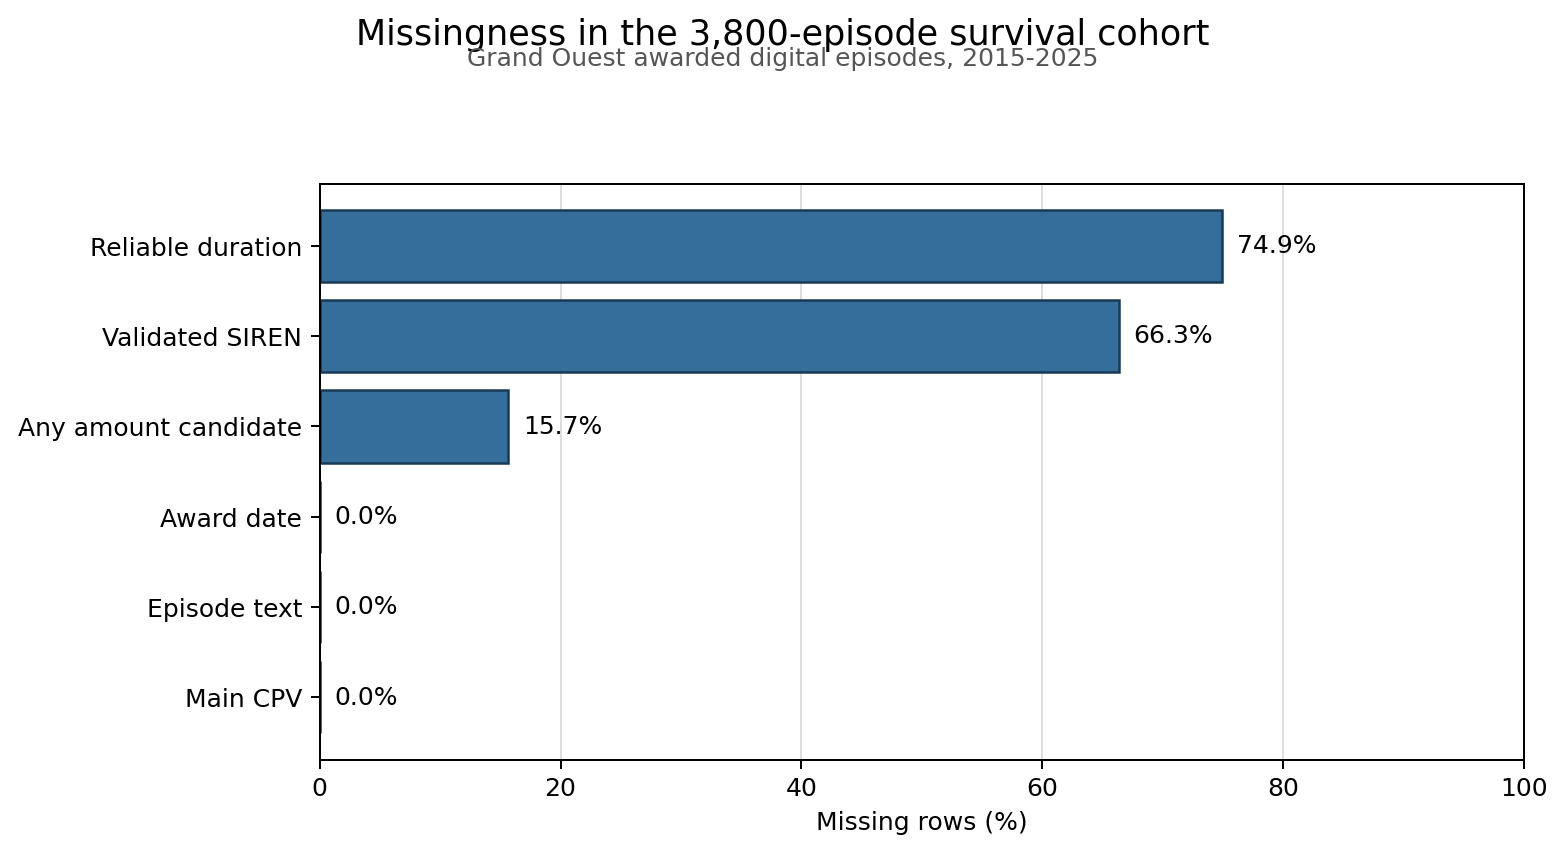
\includegraphics[width=0.8\linewidth]{figures/appB_missingness.png}
\caption{Completeness of the key cohort variables. Validated buyer identifiers and reliable durations are the
two fields whose absence shapes the methodology: the first forces a name-based fallback in buyer blocking,
the second rules out any duration-conditioned event definition.}
\label{fig:appb-missing}
\end{figure}

\begin{figure}[htbp]
\centering
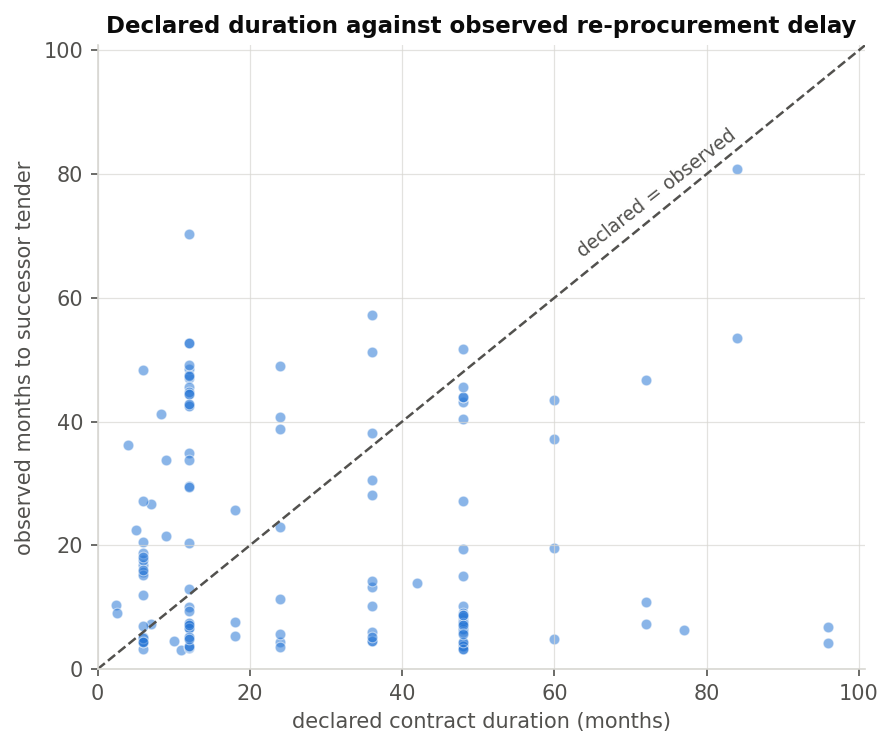
\includegraphics[width=0.8\linewidth]{figures/appB_duration_vs_observed.png}
\caption{Declared contract end against observed successor timing, for the episodes that carry both. Only
21.8\,\% of these contracts show an observable successor within six months of their declared end, and the
median absolute discrepancy is 21.1 months. This is the empirical basis for excluding declared duration from
the event definition rather than using it to bound the renewal window.}
\label{fig:appb-duration}
\end{figure}
